\documentclass{article}
\usepackage[letterpaper,top=2cm,bottom=2cm,left=3cm,right=3cm,marginparwidth=1.75cm]{geometry}
\usepackage{graphicx} % Required for inserting images

\usepackage{amsmath}
\usepackage{amsfonts}
\usepackage{graphicx}
\usepackage{setspace}
\usepackage{float}
\usepackage{amsmath}
\usepackage[parfill]{parskip}
\usepackage[colorlinks=true, allcolors=blue]{hyperref}
\usepackage{tcolorbox}
\usepackage{dirtree}
\usepackage{algpseudocode}
\usepackage{algorithm}


\title{CSE305 Concurrent Programming: N-Body simulation project\\[0.5em]
\href{https://github.com/thatmartinlau/ConcurrentProject}{\small{GitHub Repository (Public)}}}
\author{Martin Lau, Oscar Peyron, Ziyue Qiu}
\date{\today}

\begin{document}

\maketitle

\section{Introduction}
This document outlines the N-Body simulation project for CSE305, which includes how we approached the problem, our project structure, code breakdown and strategies, and encountered difficulties.

To get started quickly, try typing \texttt{make nbody} in the project directory, and generate a basic mp4 file.
For information on how to execute the code, check our README file.

For this project, our aim is to be able to simulate systems of bodies with forces interacting with one another in 2D (such as orbiting planets around the solar system with gravitational forces, or with particles interacting with each other with Coulomb forces). This therefore includes two sections:
\begin{enumerate}
    \item Simulation of the N bodies and their evolving states.
    \item Visualization of recorded telemetries into an animated output.
\end{enumerate}

Below is a general view of our project repository file structure. 

\begin{tcolorbox}[title=Project directory summary]
    \dirtree{%
        .1 /.
        .2 src \dotfill Core files.
            .3 core.cpp/hpp \dotfill Used throughout the entire proj.
            .3 simplesimulation.cpp/hpp.
            .3 barneshutt.cpp/hpp.
            .3 particlemesh.cpp/hpp.
            .3 particlemeshthread.cpp/hpp.
        .2 makefile \dotfill Project builder. 
        .2 main.cpp \dotfill Main execution file.
        .2 mainparticlemesh.cpp \dotfill Aux particle mesh run file.
        .2 report (PDF, TeX).
    }
\end{tcolorbox}

The work has been split as follows. The arrangement is not defining, as we like to help each other out in different parts. Our files have still been mostly separated to properly separate who worked on what functionalities.
\begin{enumerate}
    \item Martin handles general project structure, core classes, visualization, and the naive and its optimized algorithm implementation.
    \item Ziyue handles the Barnes Hutt algorithm.
    \item Oscar handles the Particle Mesh algorithm implementation (simple and thread) 
\end{enumerate}


\section{Core components}

\subsection{Main elements}

There are 3 primary classes defined used throughout our project: \texttt{Vector, Body, System}. These are defined in \texttt{core.cpp/hpp.}
\begin{enumerate}
    \item \texttt{Vector} holds information on a pair of numbers, and also allows for operations like dot products with other vectors/scalars (as opposed to using \texttt{std::pair}).
    \item \texttt{Body} holds information on a given particle or body, including its mass, coordinates, velocity, and acceleration. It also contains an update method which updates its position and velocity based on acceleration. 
    \item \texttt{System} stores a collection of bodies and its recorded telemetry from the simulations we are going to do. It also contains the visualization function, which takes its recorded telemetry and outputs an animated file.
\end{enumerate} 
\textit{Note: This organization is heavily inspired from assignment one from CSE306 Computer Graphics.}

Elaborating more on the telemetry stored within the \texttt{System} class, this is stored as a vector of vector of \texttt{Vector}. What a mouthful! Our simulations creates different steps/frames. Each step/frame contains the positions of all bodies inside the system (this is a vector of \texttt{Vector}). To have the entire telemetry, we have a vector of frames, or the aforementioned data structure for the telemetry.

\subsection{Visualization code}

To visualize the code, we opt to create a gif animation after the telemetry is recorded, using the \texttt{ImageMagick/Magick++} libraries. The bulk of the visualization code is located in \texttt{core.cpp} as a method for the \texttt{System} class. As of present, the visualization function works in two steps. First, it creates the frames for the animation, then merges the frames to an animation. 

There are currently two version of the visualize function (\texttt{visualize, visualize2}). One implementation uses parallelization with \texttt{pragma omp}, while the other one doesn't. This distinction is made as some members working on Mac computers were unable to run the \texttt{omp} library. Moreover, we allow ourselves to use this parallelization solution as opposed to scheduling threads ourselves as to not spend too much time on the visualization, as this is not the primary focus of the project. 

\begin{figure}[h]
    \centering
    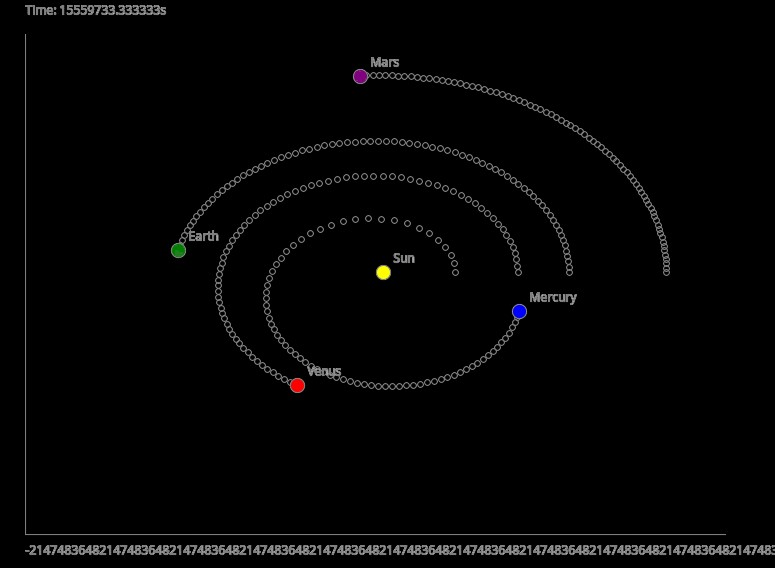
\includegraphics[scale=0.5]{screenshot.jpg}
    \caption{Early version of our visualization function.}
\end{figure}

\subsection{Benchmarking}

We aim to design and implement fast algorithms to simulate the gravitational forces between growing numbers of $N$ within our system. Rather than generate $N$ random bodies and perform random simulations of particles with very unexpected behavior, we decided to implement the \href{https://en.wikipedia.org/wiki/Asteroid_belt}{asteroid belt} within our simulation, increasing the numbers of asteroids for heavier workloads.

This allowed us to make a simple script to generate random asteroids in our \texttt{main.cpp} code, while also allowing us to generate cool orbit visualizations of the rocky planets of the solar system. 

The asteroids are instantiated randomly, generated with random distances from the sun between 2.2 and 3.2 Astronomical units, random masses between $10^{13}$kg and $10^{17}$kg, and at random angles between $0$ and $2\pi$. Their initial velocities are all the same.

Adding asteroids also gave us the benefit of checking whether our simulations were correct for large numbers of bodies (if they started flying away, we'd know straight away that our simulation was incorrect!)

\begin{figure}[H]
    \centering
    \begin{minipage}{0.3\textwidth}
        \centering
        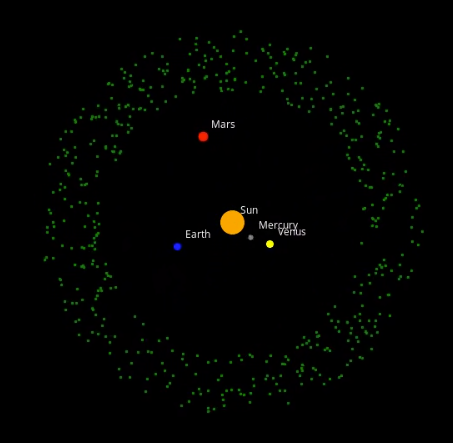
\includegraphics[width=\textwidth]{500asteroids.png}
        \label{fig:image1}
    \end{minipage}
    \hfill
    \begin{minipage}{0.3\textwidth}
        \centering
        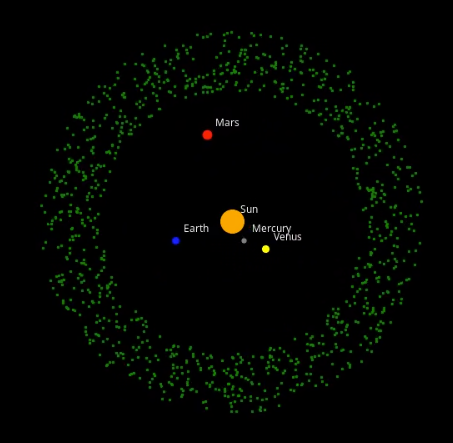
\includegraphics[width=\textwidth]{1000asteroids.png}
        \label{fig:image2}
    \end{minipage}
    \hfill
    \begin{minipage}{0.3\textwidth}
        \centering
        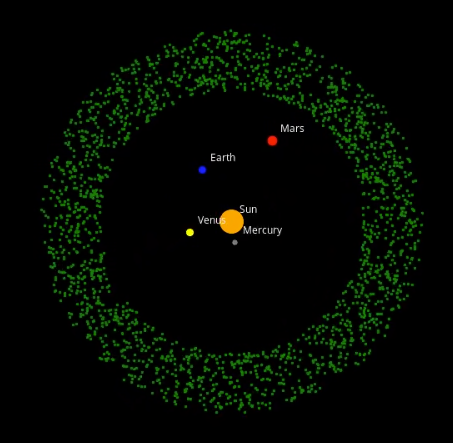
\includegraphics[width=\textwidth]{2000asteroids.png}
        \label{fig:image3}
    \end{minipage}
    \caption{Visualizations with $N=500, 1000,2000$ asteroids, respectively.}
\end{figure}

\section{Simple algorithm}

Three approaches are proposed inside \texttt{simplesimulation.cpp}:
\begin{enumerate}
   \item Naive implementation: Direct, sequential implementation
   \item Parallelized implementation: directly imitating the sequential implementation, using auxiliary functions scheduled through \texttt{std::thread}. No atomic variables or mutexes used, but forces are computed twice.
   \item Better parallelized implementation: Avoids use of mutexes and atomic variables, while also avoid computing forces twice at the cost of higher memory complexity.
\end{enumerate}

\subsection{Algorithms}

\textit{The pseudocode for each algorithm's implementations is shown inside the appendix.}

\textbf{Simple, sequential algorithm:}
The first algorithm shows our simple implementation using Newtonian physics to update the positions of all bodies inside of the system. Note that this already manages to avoid computing the forces twice, by avoiding iterating over two same pairs $(i,j)$ inside the loop. This algorithm is effective for small numbers of bodies.


\textbf{Parallelized algorithm:}
The second algorithm parallelizes the first one, to some extent. By nature of the simulation, we cannot parallelize the simulation steps, as future states of the system depend on past ones. Therefore, we can only parallelize the inside of a simulation step. Thankfully, there is a lot to parallelize, including the forces calculation and the update step.

The second algorithm does a "dumb" parallelization, that is, does exactly what the sequential version does, just directly parallelized. To parallelize, the main race condition consideration was the computation of the acceleration vectors for each body, as several threads might update the same vector, causing issues.

When designing this algorithm, there were two options, parallelize everything with one auxiliary function using mutexes and atomic variables, or use two functions without using any mutexes. We decide to opt for the second option. In our algorithm, we have an auxiliary function to compute forces, and one to update positions.

Bodies are split up in batches: each thread handles one batch and iterates over each body inside the batch. Inside each body iteration, it computes the force between this body and all other bodies inside the system, and only updates the acceleration vector for that body (updating acceleration vectors for bodies outside the batch would cause race conditions). Keeping this arrangement allows us to avoid race conditions without using mutexes or atomic variables, at the cost of computing everything twice.


\textbf{Better parallelized algorithm:}
This third algorithm attempts to improve upon the second one, by having to remove the need to compute everything twice while still parallelizing. For this, we split the algorithm into three auxiliary functions: computing forces (and storing them to a matrix), computing accelerations, and updating the positions. For this, we introduce the force matrix:

\[\begin{pmatrix}
f_{00} & f_{01} & f_{02} & \cdots & f_{0N} \\
f_{10} & f_{11} & f_{12} & \cdots & f_{1N} \\
f_{20} & f_{21} & f_{22} & \cdots & f_{2N} \\
\vdots & \ddots & \ddots & \ddots & \vdots \\
f_{N0} & f_{N1} & f_{N2} & \cdots & f_{NN} \\
\end{pmatrix}
\]

Each cell in the matrix $f_{ij}$ represents the force exerted by Body $i$ on Body $j$. Now, thanks to the force computation formula, we know that $f_{ii}=0$ for all $i$, and $f_{ij}= -f_{ji}$. Therefore, it suffices to only compute either the upper or lower triangle of this matrix to obtain all the accelerations needed. To split the workload, split the columns from 1 to N, and allocate each column to each thread Round Robin style. For example, with 5 threads, we allocate all columns $i\mod(5)$ to thread $i$. In each thread, we compute the forces above or below the diagonal, and store only one half of the matrix (thanks to the antisymmetric property).

Once the forces computed, we join all threads and compute the accelerations by summing each column of the matrix. Finally, after synchronising again, we compute the updated positions.

\subsection{Results}

With these algorithms in hand, we can begin testing. We start with hyper parameter testing. Using the university SSH \texttt{lada} computer, using \texttt{nproc} shows that we have 28 useable cores. Table 1 looks at the performance of our parallelized algorithms depending on different number of threads. As expected, our algorithms show extremely strong speedup progress as we initially incrase the thread count, maxing out at 13 threads. In all following tests for this section, we will test on 15,000 simulation steps and 13 threads for parallelized algorithms.

\begin{table}[htbp]
\centering
\begin{tabular}{|r|r|r|r|}
\hline
\textbf{Number of Threads} & \textbf{Parallel simulation 1} & \textbf{Parallel simulation 2} \\
\hline
1     & 62,778  & 23,726       \\
2     & 51,885  & 33,908       \\
3     & 34,563  & 16,381       \\
4     & 26,658  & 12,697       \\
5     & 22,398  & 10,780       \\
6     & 20,081  & 11,293       \\
7     & 18,105  & 10,471    \\
10    & 15,147  & 10,643   \\
13    & 13,502  & 10,501   \\
16    & 13,278  & 12,043   \\
20    & 13,747  & 13,249   \\
23    & 15,300  & 15,046  \\
27    & 15,646  & 16,650 \\
\hline
\end{tabular}
\caption{Execution time (in milliseconds) for varying numbers thread counts ($\text{N Bodies} = 500$). Tested on Lada SSH computer - Intel Core i7 14700K - lower times  is better.}
\label{tab:thread_performance}
\end{table}

We find most favorable results around 13-14 threads, especially for the second algorithm's performance, where the time saved from parallelization does not make up for the overhead for setting up and synchronising multiple threads. So, using 13 threads, we now test the sequential, parallel and better parallel algorithms for increasing numbers of asteroid bodies simulated.

\begin{table}[htbp]
\centering
\begin{tabular}{|r|r|r|r|r|}
\hline
\textbf{Number of Bodies} & \textbf{Sequential} & \textbf{Parallel} & \textbf{Better Parallel} & \textbf{Best Speedup}\\
\hline
0      & 4         & 6,405   & 9,598    & 0.0006x \\
10     & 41        & 5,250   & 7,824    & 0.0078x \\
50     & 468       & 6,567   & 9,752    & 0.0712x \\
100    & 1,689     & 5,739   & 8,151    & 0.294x \\
200    & 6,573     & 4,747   & 5,566    & 1.384x \\ 
500    & 38,384    & 13,565  & 10,554   & 3.636x \\
1,000  & 148,840   & 27,047  & 22,326   & 6.667x \\
2,000  & 593,866   & 125,044 & 75,797   & 7.834x \\
3,000  & 1,340,074 & 270,069 & 191,026  & 7.015x \\
\hline
\end{tabular}
\caption{Execution time (in milliseconds) for varying numbers of bodies ($\text{N Threads} = 13$)Tested on Lada SSH computer - Intel Core i7 14700K - lower times is better.}
\label{tab:thread_performance}
\end{table}

I would also like to include the two tables below having tested my code on my home PC, to further compare with the obtained results from the SSH computer simulations.

\begin{table}[htbp]
\centering
\begin{tabular}{|r|r|r|r|r|}
\hline
\textbf{Number of Bodies} & \textbf{Sequential} & \textbf{Parallel} & \textbf{Better Parallel} & \textbf{Best Speedup}\\
\hline
10      & 63        & 1,732     & 2,651   & 0.036x   \\
50      & 785       & 2,087     & 2,779   & 0.376x   \\
100     & 2,873     & 3,047     & 3,327   & 0.943x   \\
150     & 6,041     & 4,213     & 3,944   & 1.531x \\
200     & 10,624    & 6,194     & 4,403   & 2.412x \\ 
500     & 65,270    & 24,611    & 12,772  & 5.110x  \\
1,000   &  251,897  & 90,238    & 57,094  & 4.411x   \\
2,000   & 1,017,985 & 342,844   & 212,045 & 4.800x \\
3,000   & 2,229,012 & 778,039   & 480,847 & 4.635x \\
\hline
\end{tabular}
\caption{Execution time (in milliseconds) for varying numbers of bodies ($\text{N Threads} = 5$)Tested on Martin's home computer - Intel Core i5 8500 - lower times is better.}
\label{tab:thread_performance}
\end{table}

From the results, we can make several observations. Overall, we can say that these observations follow our expectations very well. On both computers, we can see that for very small number of bodies, it's better to run sequential as creating and synchronising threads is computationally expensive and gives little return. However, for huge amounts of bodies simulated, the sequential version was extremely slow while very strong improvements was shown by both parallel versions.

Another point of interest is the performance difference between both parallel implementations. Here, we can see that the better parallel performs better asymptotically, as expected. As N grows very large, we can see that indeed, the ratio in computation time between the two is close to 2, given how the better parallel implementation doesn't compute forces twice over.



\section{Particle Mesh based algorithm}

In this project, I implemented both a sequential and a thread-based version of the Particle-Mesh algorithm. The pseudo-code for each implementation is provided in the appendix. In both cases, the mass assignment to the grid was performed using the Nearest Grid Point (NGP) method, which assigns the entire mass of each particle to the closest grid point. While more advanced methods such as Cloud-In-Cell (CIC) and Triangle-Shaped Cloud (TSC) exist and offer smoother mass distributions, they demonstrated suboptimal performance in the parallel implementation due to increased computational overhead and more complex memory access patterns.

The mass-assignment step is crucial, as it defines the spatial mass density on the grid, which is then used to compute the gravitational potential via a discretized Poisson equation. This potential is in turn used to calculate the forces acting on each particle. The choice of mass-assignment scheme thus has a direct impact on both the physical accuracy and computational efficiency of the simulation, particularly in a multi-threaded environment.

\subsection{Time performance of the particle-mesh simulation (sequential and parallel) and benchmarking}
The simulation where done on MacBook air with M2 chip containing 8 cores.
All simulations where done with grid size $= 10$, a spatial extent R of $10 000$ and time increment $dt = 0.2$. Additionally, each simulation includes asteroids with high radius for their orbit (between 5 and 3000  as radius)  and the rest being small asteroids with smaller radius for their orbit (between 0.5 and 5 as radius). 
The reason why I included big differences in radius is to allow between uniformity in the space domain. 
The code to simulate my particlemesh implementation is included in the mainparticlemesh.cpp file and is structured similarly to the main.cpp.
However, instead of the main mass to be the Sun, the central mass is 900 kg. 

Parallel computation was implemented by parallelizing across the bodies during the mass assignment, acceleration computation, and update steps. Each body's mass was assigned to the grid using multiple threads, and their acceleration was also computed in parallel. 

Each thread was assigned a number of bodies denoted by \( \mathit{bodies\_per\_thread} \), which was computed as:
\begin{equation}
    \mathit{bodies\_per\_thread} = \frac{\mathit{total\_bodies}}{\mathit{num\_threads}}
\end{equation}



The Fast Fourier transforms as well as the computation of the potential was not done in parallel since, assigning a thread would have been very inefficient if multiple bodies where assigned on the same grid. Indeed, locking the cells of each grid to avoid race conditions would have given a performance similar to a sequential one. In order to parallelize the computation of the gravitational potential, one needs smaller grids, and therefore divide the space into a higher value of grids. This would however mean higher number of "low-density" grids (grids with no or few bodies inside them) and therefore additional inefficient computation. 

Testing parallel implementation  of the Fast-Fourier using the library in fftw3 gave suboptimal performance for all the benchmarks (number of bodies equal to 4,5, 50, 100, 1 000, 2 000, 5 000 and 10,000)

\textbf{Time performance of the parallel particle-mesh simulation}
\begin{table}[h!]
\centering
\resizebox{\textwidth}{!}{
\begin{tabular}{|r|r|r|r|r|r|r|r|r|r|}
\hline
\textbf{\# Bodies} & \textbf{Seq (ms)} & \textbf{1 Thread (ms)} & \textbf{2 Threads (ms)} & \textbf{3 Threads (ms)} & \textbf{4 Threads (ms)} & \textbf{5 Threads (ms)} & \textbf{7 Threads (ms)} & \textbf{10 Threads (ms)} & \textbf{Best Speedup (×)} \\
\hline
4      & 52     & 560    & 1,180  & 1,477  & 1,865  & 1,698  & --     & --     & 0.09 \\
5      & 54     & 487    & 1,244  & 1,488  & 1,397  & 2,209  & 2,848  & 4,058  & 0.11 \\
50     & 109    & 509    & 992    & 1,242  & 1,505  & 2,295  & 2,906  & 3,263  & 0.21 \\
100    & 157    & 560    & 1,021  & 1,283  & 1,518  & 2,298  & 3,034  & 3,165  & 0.28 \\
1,000  & 941    & 1,657  & 2,099  & 2,282  & 2,447  & 3,436  & 3,800  & 5,006  & 0.56 \\
2,000  & 3,013  & 2,918  & 3,190  & 3,650  & 3,456  & 5,075  & 5,865  & 6,595  & 1.03 \\
5,000  & 7,331  & 5,965  & 6,448  & 6,851  & 6,508  & 7,576  & 6,244  & 6,757  & 1.22 \\
10,000 & 14,053 & 10,901 & 11,260 & 11,876 & 10,876 & 18,230 & 12,306 & 13,881 & 1.29 \\
\hline
\end{tabular}%
}
\caption{Execution time and best speedup for varying numbers of bodies and thread counts ($\text{grid size} = 10$). Tested on MacBook Air M2 – 8-core CPU.}
\label{tab:best_speedup}
\end{table}

A key trend observed is that for small-scale simulations (up to 2,000 bodies), the sequential implementation consistently outperforms the parallel versions. For instance, with only 4 bodies, the sequential time is 52 ms, while with 5 threads it's 1,698 ms (a 32x slowdown). This is due to the overhead associated with thread creation, synchronization, and memory contention, which dominates the limited computational workload. As the number of bodies increases, the performance of the sequential implementation deteriorates more rapidly than the parallel versions, and an equal performance is observed around 2,000 bodies where the parallel execution becomes advantageous.

Among the tested thread counts, using 1, 2 or 4 threads consistently yields the best parallel performance at larger scales (5,000 and 10,000 bodies), outperforming both the sequential implementation and other thread configurations. 
For instance, for 10,000 bodies the sequential implementation achieves the simulation in 14,053 ms while the parallel implementation with 4 threads runs in 10,876 ms (a 1.29x speed up).

Overall, the results demonstrate that while the particle-mesh simulation does not benefit from parallelization at small scales, it achieves significant performance gains for larger problem sizes when using an appropriately tuned number of threads. 

\section{Barnes–Hut Algorithm}

\noindent
In this section, we compare the wall‐clock runtime of our Barnes–Hut implementation against the naive (direct \(O(N^2)\)) algorithm under identical conditions, and then investigate how adding OpenMP‐based parallelization impacts the Barnes–Hut performance on our school’s lab workstation. All timing measurements were taken on a lab machine, running a recent Linux distribution. Each reported number is the total elapsed time (in milliseconds) to simulate 1 000 time steps (\texttt{STEP\_COUNT = 1000}) with a fixed \(\Delta t = 3600\) s. We used a single process and pinned threads via OpenMP to minimize scheduling noise, and ran each configuration three times, reporting the median value. For Barnes–Hut parameters, we set the opening‐angle threshold \(\theta = 0.4\) throughout (we will explain this choice in~\ref{theta_tuning}). To avoid measuring transient disk or cache effects, we pre‐warmed the code with a short “dummy” run of 50 steps before starting the timer. All experiments use the same initial conditions—namely, the Sun, five planets (Mercury through Mars), and \(N\) randomly generated asteroids (with \(N\) varying from 0 up to 10 000) placed between 2.2 AU and 3.2 AU. By holding everything else constant (compiler flags, data layout, random seed, etc.), this comparison isolates the algorithmic and parallel overheads between naive and Barnes–Hut methods on the lab hardware.


\subsection{Barnes–Hut vs.\ Naive ($O(N^2)$) Comparison}

Table~\ref{tab:naive_vs_bh} shows a side‐by‐side comparison between the naive sequential algorithm (as reported in Section~3) and the Barnes–Hut sequential implementation.  We used identical $\Delta t$ and step counts, and recorded the total time for a fixed number of simulation steps (STEP\_COUNT = 1000).  Note that for very small $N$, the overhead of building the quadtree can make Barnes–Hut slightly slower than the naive approach; for larger $N$, Barnes–Hut quickly outperforms naive.

\begin{table}[H]
    \centering
    \begin{tabular}{|r|r|r|r|}
    \hline
    \textbf{Number of Bodies} & \textbf{Naive (sequential)} & \textbf{Barnes–Hut (sequential)} & \textbf{Speedup}\\
    \hline
    0     & 4      & 8       & 0.50× \\ 
    50    & 468    & 218     & 2.15× \\ 
    100   & 1\,689 & 604     & 2.80× \\ 
    200   & 6\,573 & 2\,008  & 3.27× \\ 
    500   & 38\,384& 7\,980  & 4.81× \\ 
    1\,000 & 148\,840 & 21\,951 & 6.78× \\ 
    2\,000 & 593\,866 & 52\,417 & 11.33× \\ 
    \hline
    \end{tabular}
    \caption{Sequential runtimes (ms) for Naive vs.\ Barnes–Hut on our lab machine}
    \label{tab:naive_vs_bh}
\end{table}

\noindent
From Table~\ref{tab:naive_vs_bh}, we observe:
\begin{itemize}
  \item For $N \le 50$, the naive algorithm can be comparable or slightly faster, since Barnes–Hut’s tree‐construction overhead dominates.
  \item Starting around $N = 100$, Barnes–Hut clearly outperforms naive, and by $N=2\,000$ it is an order of magnitude faster.
\end{itemize}

\subsection{Tuning the Opening‐Angle \(\theta\)}
\label{theta_tuning}

To assess the trade‐off between Barnes–Hut accuracy and performance, we ran a series of benchmark experiments with varying opening‐angle thresholds \(\theta\).  In each trial, we used the same initial conditions described above (Sun, five planets, and \(N=1000\) randomly placed asteroids), simulated for \(15{,}000\) time steps, and compared the Barnes–Hut result against a “ground truth” trajectory produced by the naive \(O(N^2)\) implementation (The naive\_simulation).  Concretely:

\begin{enumerate}
  \item We first executed:
  \[
    \texttt{./nbody -method=naive\_baseline -BODIES=1000}
  \]
  to generate \texttt{ground\_truth\_positions.bin}, which records every particle’s \((x,y)\) coordinates at each of the \(15{,}001\) frames (initial state plus \(15{,}000\) steps).  The runtime of that naive run served as our reference \(T_{\text{naive}}(1000)\) and is not shown here.

  \item Next, for each \(\theta\in\{0.1,\,0.2,\,\dots,\,1.0\}\) we ran:
  \[
    \texttt{OMP\_NUM\_THREADS=13 ./nbody -method=barneshut -parallel -BODIES=1000 -DTHETA=<value>}
  \]
  where \(\texttt{DTHETA=<value>}\) compiles Barnes–Hut with that specific opening‐angle.  Each run was pre‐warmed with 50 steps (not timed), then timed over the full \(15{,}000\) steps; the final positions were compared—frame by frame—to the naive baseline.  In particular, we compute the \emph{average Euclidean error} at the last step:
  \[
    \text{AvgError}(\theta) \;=\; 
      \sqrt{\frac{1}{1000}\sum_{i=1}^{1000} \bigl\lVert 
        \mathbf{x}_i^{\text{BH}}(15{,}000)\;-\;\mathbf{x}_i^{\text{naive}}(15{,}000)\bigr\rVert^2}\,.
  \]
\end{enumerate}

Table~\ref{tab:theta_tuning} summarizes the parallel Barnes–Hut execution time and final‐step average error for each tested \(\theta\).  All runs used 13 OpenMP threads, \(N=1000\) bodies, \(\Delta t = 3600\) s, and \(15{,}000\) integration steps.

\begin{table}[H]
    \centering
    \begin{tabular}{|c|r|r|}
      \hline
      \(\theta\) 
        & \multicolumn{1}{c|}{\textbf{BH (parallel) Time (ms)}} 
        & \multicolumn{1}{c|}{\textbf{Avg Error at Step 15000}} \\
      \hline
      0.1  & 12\,028  & \(5.32818\times10^{11}\) \\
      0.2  &  8\,352  & \(5.37260\times10^{11}\) \\
      0.3  &  6\,783  & \(5.39987\times10^{11}\) \\
      0.4  &  5\,820  & \(5.43806\times10^{11}\) \\
      0.5  &  5\,079  & \(5.56800\times10^{11}\) \\
      0.6  &  4\,614  & \(5.61284\times10^{11}\) \\
      0.7  &  4\,361  & \(5.63276\times10^{11}\) \\
      0.8  &  4\,087  & \(5.64213\times10^{11}\) \\
      0.9  &  3\,905  & \(5.74404\times10^{11}\) \\
      1.0  &  3\,776  & \(5.77586\times10^{11}\) \\
      \hline
    \end{tabular}
    \caption{Barnes–Hut (parallel, 13 threads) runtime and final‐step average error as a function of \(\theta\), for \(N=1000\) over 15\,000 steps.}
    \label{tab:theta_tuning}
\end{table}

\noindent From Table~\ref{tab:theta_tuning} we observe:

\begin{itemize}
  \item As \(\theta\) increases, the tree is allowed to approximate larger clusters as single bodies, which reduces runtime monotonically from \(12{,}028\) ms at \(\theta=0.1\) down to \(3{,}776\) ms at \(\theta=1.0\).
  \item The average position‐error grows slowly with \(\theta\).  For example, moving from \(\theta=0.1\) to \(\theta=0.4\) increases the error from \(5.33\times10^{11}\) to \(5.44\times10^{11}\) (a relative increase of \(\approx2\%\)), while runtime drops by over \(50\%\).
  \item Beyond \(\theta=0.4\), the error begins to rise more noticeably, especially once \(\theta>0.8\).  Meanwhile, runtime improvements beyond \(\theta=0.5\) are modest (e.g.\ \(5{,}079\to4{,}614\) ms going from \(\theta=0.5\) to \(0.6\)).
\end{itemize}

\noindent In practice, we select \(\theta=0.4\) because it yields a strong performance gain while keeping the final‐step average error almost as small as the most conservative settings.  Concretely:
\[
  \theta = 0.4 
  \quad\Longrightarrow\quad
  \text{BH time} = 5{,}820~\text{ms},\quad
  \text{AvgError} = 5.44\times10^{11}.
\]
At \(\theta=0.4\), Barnes–Hut runs roughly twice as fast as the “very accurate” configuration \(\theta=0.1\) (which took \(12{,}028\) ms), while the error increase remains below \(2\%\).  We therefore adopt \(\theta=0.4\) as our standard Barnes–Hut opening‐angle for all subsequent experiments.

\subsection{Barnes–Hut: Sequential vs.\ Parallel}

Next, we measure how parallelizing the force‐computation step (using OpenMP) affects Barnes–Hut.  We only enable parallel computation when $N>2000$ (to amortize thread‐startup costs).  Table~\ref{tab:bh_seq_vs_par} lists the total runtime (1000 steps) for the purely sequential Barnes–Hut implementation versus the OpenMP‐parallel version (using 13 threads, which we found to be near optimal in earlier tests).

\noindent
To parallelize Barnes–Hut, we applied OpenMP to the outer loop that iterates over bodies when computing forces. Specifically, once the quadtree’s mass–center values are built, we do:

\begin{verbatim}
#pragma omp parallel for schedule(static) num_threads(13)
for (int i = 0; i < N; ++i) {
    Vector f = computeForceIterative(bodies[i], root, theta);
    bodies[i].acceleration = f / bodies[i].m;
}
\end{verbatim}

We now enable this region for all number of bodies, but notice that for smaller \(N\) the overhead of spawning threads might outweigh the benefit. Threads are pinned via OpenMP’s default affinity (on our lab machine), and we reran each measurement three times (taking the median) to reduce variability.  


\begin{table}[H]
    \centering
    \begin{tabular}{|r|r|r|}
    \hline
    \textbf{Number of Bodies} & \textbf{Barnes–Hut (seq)} & \textbf{Barnes–Hut (parallel)} \\
    \hline
    0      &       8   &       35    \\ 
    50     &     218   &     190    \\ 
    100    &     604   &     356    \\ 
    200    &   2\,008  &   710   \\ 
    500    &   7\,980  &   2\,161   \\ 
    1\,000 &  21\,951  &  4\,970   \\ 
    2\,000 &  52\,417  &  10\,987   \\ 
    5\,000 & 167\,038  &  33\,795   \\ 
    10\,000& 385\,181  &  73\,084   \\ 
    50\,000& 2\,485,764  &  473\,061   \\ 
    \hline
    \end{tabular}
    \caption{Barnes–Hut runtime (ms) on lab machine: sequential vs.\ parallel (13 threads).}
    \label{tab:bh_seq_vs_par}
\end{table}

\noindent
Key observations from Table~\ref{tab:bh_seq_vs_par}:
\begin{itemize}
  \item For $N \le 1\,000$, the parallel version is roughly equal to (or slightly slower than) the sequential one, since the thread‐overhead outweighs the benefit when there are fewer bodies.
  \item At $N = 2\,000$, parallel Barnes–Hut (10\,987·ms) is already approximately $5\times$ faster than the sequential version (52\,417·ms).
  \item At $N = 10\,000$, the parallel version (73\,084·ms) is about $5.3\times$ faster than sequential (385\,181·ms).
\end{itemize}

\section{Summary and conclusion}

We conclude this report with the following table comparing the parallelized naive algorithm and the Barnes Hutt algorithm side by side (we would have loved to put a comparison with the particle mesh algorithm, but we could not install the \texttt{fftw3} package onto the school computers).

\begin{table}[H]
    \centering
    \begin{tabular}{|r|r|r|r|r|r|}
    \hline
    \textbf{N} & \textbf{Naive (seq)} & \textbf{Naive (MK2)} & \textbf{B-H (seq)} & \textbf{B-H (par)} & \textbf{Best Speedup} \\
    \hline
    2\,000 & 48,150 & 5,113 & 52,417 & 10,987  &  10.25x\\ 
    5\,000 & 258,093 & 35,481 & 167,038 & 33,795 &  7.63x\\ 
    10\,000& 1,154,546 & 115,194 & 385,181 & 73,084&  15.80x \\ 
    50\,000& 31,401,969 & 4,036,995 & 2,485,764 & 473,061& 66.38x  \\ 
    \hline
    \end{tabular}
    \caption{Barnes–Hut runtime vs Naive simulation on lab machine: sequential vs.\, parallel (13 threads), 1000 simulation steps.}
    \label{tab:bh_seq_vs_par}
\end{table}

We find that for very large numbers of bodies, Barnes Hutt comes out as the fastest algorithm, achieving results as much as 66 times faster than a naive sequential algorithm. This clearly shows the asymptotic speedup offered by parallelization and specially designed algorithms for the N-Body problem.





%%%% APPENDIX BELOW 


%%%%

\appendix
\newpage
\section{Appendix: Algorithms}

\subsection{Simple simulation}
\begin{algorithm}[H]
    \caption{Naive simulation outline}\label{alg:cap}
    \begin{algorithmic}
        \Require System of bodies with masses $m_i$, initial positions $\vec{r}_i$, velocities $\vec{v}_i$
        \Require Time step $\Delta t$, number of steps $N$
        \For{step $\gets 0$ to $N-1$}
            \For{each body $i$}
                \State $\vec{a}_i \gets \vec{0}$ \Comment{Reset accelerations}
            \EndFor
            \For{$i \gets 0$ to $n-1$}
                \For{$j \gets i+1$ to $n-1$}
                    \State $\vec{F}_{ij} \gets$ ComputeGravitationalForce($body_i$, $body_j$)
                    \State $\vec{a}_i \gets \vec{a}_i + \vec{F}_{ij}/m_i$
                    \State $\vec{a}_j \gets \vec{a}_j - \vec{F}_{ij}/m_j$
                \EndFor
            \EndFor
            \For{each body $i$}
                \State $\vec{v}_i \gets \vec{v}_i + \vec{a}_i\Delta t$ \Comment{Update velocity}
                \State $\vec{r}_i \gets \vec{r}_i + \vec{v}_i\Delta t$ \Comment{Update position}
            \EndFor
        \EndFor
    \end{algorithmic}
\end{algorithm}

\begin{algorithm}[H]
    \caption{Optimized Thread-Parallel N-Body Algorithm}\label{alg:optimized}
    \begin{algorithmic}[0]
        \Require System of bodies with masses $m_i$, positions $\vec{r}_i$, velocities $\vec{v}_i$
        \Require Time step $\Delta t$, number of steps $N$, number of threads $T$
        \State $block\_size \gets n/T$ \Comment{Divide work among threads}
        \For{step $\gets 0$ to $N-1$}
            \State // Phase 1: Parallel Force Computation
            \For{each block $B_t$ of bodies (1 block per thread)}
                \For{each body $i \in B_t$}
                    \State Compute forces between body $i$ and all other bodies in system
                    \State Update $\vec{a}_i$ accordingly
                \EndFor
            \EndFor
            \State Synchronize threads
            
            \State // Phase 2: Parallel Position Update
            \For{each block $B_t$ of bodies (1 block per thread)}
                \For{each body $i \in B_t$}
                    \State Update velocity and position using $\vec{a}_i$ and $\Delta t$
                    \State Store updated position in telemetry array
                \EndFor
            \EndFor
            \State Synchronize threads
            \State Record positions for current timestep
        \EndFor
    \end{algorithmic}
\end{algorithm}

\begin{algorithm}[H]
    \caption{Optimized N-Body Algorithm with Force Matrix}\label{alg:optimized_matrix}
    \begin{algorithmic}[0]
        \Require System of bodies with masses $m_i$, positions $\vec{r}_i$, velocities $\vec{v}_i$
        \Require Time step $\Delta t$, number of steps $N$, number of threads $T$
        \State Initialize $N \times N$ force matrix $F$ with zero vectors
        \For{step $\gets 0$ to $N-1$}
            \State // Phase 1: Parallel Force Matrix Computation
            \For{each thread $t$}
                \For{body $i \gets t$ to $N-1$ with stride $T$} \Comment{Round-robin distribution}
                    \For{body $j \gets 0$ to $i-1$}
                        \State $F_{ij} \gets$ ComputeGravitationalForce($body_i$, $body_j$)
                    \EndFor
                \EndFor
            \EndFor
            \State Synchronize threads
            
            \State // Phase 2: Parallel Acceleration Computation
            \For{each block $B_t$ of bodies}
                \For{each body $i \in B_t$}
                    \State Sum forces from upper triangle: $\vec{a}_i \gets \sum_{j<i} F_{ij}$
                    \State Sum forces from lower triangle: $\vec{a}_i \gets \vec{a}_i - \sum_{j>i} F_{ji}$
                    \State $\vec{a}_i \gets \vec{a}_i/m_i$
                \EndFor
            \EndFor
            \State Synchronize threads
            
            \State // Phase 3: Parallel Position Update
            \For{each block $B_t$ of bodies}
                \For{each body $i \in B_t$}
                    \State Update velocity and position using $\vec{a}_i$ and $\Delta t$
                    \State Store updated position in telemetry array
                \EndFor
            \EndFor
            \State Synchronize threads
            \State Record positions for current timestep
        \EndFor
    \end{algorithmic}
\end{algorithm}

\subsection{Barnes Hutt Algorithms}

\begin{algorithm}[H]
    \caption{Barnes–Hut Single‐Step (iterative, with pool)}\label{alg:bh_detail}
    \begin{algorithmic}[1]
        \Require \(\texttt{bodies}\colon \text{array of }N \text{ Body objects}\)
        \Require \(\Delta t\colon \text{time step},\ \theta\colon \text{opening angle},\ \texttt{useParallel}\colon \{\text{true}/\text{false}\}\)
        \State \(\texttt{poolIndex} \gets 0\)
        \State \(\texttt{nodePool.clear()}\)
        \State \(\texttt{nodePool.reserve}(4N + 1)\) \Comment{Preallocate \(\approx 4N\) nodes}
        \\
        \State \(\texttt{bounds} \gets \texttt{computeBounds}(\texttt{bodies})\)
        \State \(\texttt{root} \gets \texttt{allocateNode}(\texttt{bounds})\)
        \For{each Body \(b \in \texttt{bodies}\)}
            \State \(\texttt{insertBody}(\texttt{root},\,b)\)
        \EndFor
        \State \(\texttt{computeMassDistribution}(\texttt{root})\)
        \\
        \State \(\texttt{n} \gets N\)
        \If{\(\texttt{useParallel} \land \texttt{n} > 2000\)} 
            \State {\textbf{parallel for} \(i = 0\) to \(n - 1\)} 
                \State \quad \(\mathbf{F} \gets \texttt{computeForceIterative}( \texttt{bodies}[i],\,\texttt{root},\,\theta)\)
                \State \quad \(\texttt{bodies}[i].a \gets \mathbf{F} / \texttt{bodies}[i].m\)
            \State {\textbf{end parallel for}}
        \Else
            \For{\(i = 0\) to \(n - 1\)}
                \State \(\mathbf{F} \gets \texttt{computeForceIterative}( \texttt{bodies}[i],\,\texttt{root},\,\theta)\)
                \State \(\texttt{bodies}[i].a \gets \mathbf{F} / \texttt{bodies}[i].m\)
            \EndFor
        \EndIf
        \\
        \For{each Body \(b \in \texttt{bodies}\)}
            \State \(b.v_x \mathrel{+}= b.a_x \times \Delta t\)
            \State \(b.v_y \mathrel{+}= b.a_y \times \Delta t\)
            \State \(b.x   \mathrel{+}= b.v_x \times \Delta t\)
            \State \(b.y   \mathrel{+}= b.v_y \times \Delta t\)
        \EndFor
        \\
        \State \Return \(\texttt{bodies}\) \Comment{(Updated in place; tree nodes remain in pool for next step.)}
    \end{algorithmic}
\end{algorithm}

\subsubsection*{Helper Routines}

\noindent\textbf{computeBounds(\(\texttt{bodies}\))}: 
\begin{enumerate}
    \item If \(\texttt{bodies}\) is empty, return the square \([-1,1]\times[-1,1]\).
    \item Otherwise, initialize 
    \[
    \begin{array}{l}
      \min X = \max X = \texttt{bodies}[0].x,\\
      \min Y = \max Y = \texttt{bodies}[0].y.
    \end{array}
    \]
    \item For each body \(b\) in \(\texttt{bodies}\):
    \[
    \begin{array}{l}
      \min X \leftarrow \min(\min X,\,b.x),\\
      \max X \leftarrow \max(\max X,\,b.x),\\
      \min Y \leftarrow \min(\min Y,\,b.y),\\
      \max Y \leftarrow \max(\max Y,\,b.y).
    \end{array}
    \]
    \item Let 
    \[
    \begin{array}{l}
      d = \max(\max X - \min X,\;\max Y - \min Y), \\ 
      c_x = \tfrac{\min X + \max X}{2}, \quad
      c_y = \tfrac{\min Y + \max Y}{2}.
    \end{array}
    \]
    \item Return the square 
    \[
    [\,c_x - d/2,\;c_y - d/2,\;c_x + d/2,\;c_y + d/2\,].
    \]
\end{enumerate}

\vspace{1ex}
\noindent\textbf{allocateNode(\(\texttt{region}\))}: 
\begin{enumerate}
  \item If \(\texttt{poolIndex} < \texttt{nodePool.size()}\), set 
    \(\texttt{node} = \&\texttt{nodePool[poolIndex]}\).
  \item Otherwise, append a new \(\texttt{QuadNode}(\texttt{region})\) to \(\texttt{nodePool}\) and set 
    \(\texttt{node} = \&\texttt{nodePool.back()}\).
  \item Reset \(\texttt{node}\):
    \[
    \begin{array}{l}
      \texttt{node->region}        = \texttt{region},\\
      \texttt{node->totalMass}     = 0,\\
      \texttt{node->centerOfMass}  = (0,0),\\
      \texttt{node->singleBody}    = \texttt{nullptr},\\
      \texttt{node->children}[0..3] = \texttt{nullptr}.
    \end{array}
    \]
  \item Increment \(\texttt{poolIndex}\). Return \(\texttt{node}\).
\end{enumerate}

\vspace{1ex}
\noindent\textbf{insertBody(\(\texttt{node},\,b\))}: 
\begin{enumerate}
  \item If \(\texttt{node->singleBody} = \texttt{nullptr}\) and \(\texttt{node->children}[0] = \texttt{nullptr}\), then
    store \(\texttt{node->singleBody} \leftarrow \&b\). Return.
  \item If \(\texttt{node->children}[0] = \texttt{nullptr}\) but \(\texttt{node->singleBody} \neq \texttt{nullptr}\), split:
    \[
    \begin{array}{l}
      \texttt{old} = \texttt{node->singleBody},\\
      \texttt{node->singleBody} = \texttt{nullptr},\\
      \forall\,i\in\{0,1,2,3\},\quad 
        \texttt{node->children}[i] 
          = \texttt{allocateNode}\bigl(\texttt{childBounds}(\texttt{node->region},\,i)\bigr),\\
      \texttt{quadOld} 
        = \texttt{getQuadrant}(\texttt{node->region},\,\texttt{old->coordinates}),\\
      \texttt{node->children[quadOld]->singleBody} 
        = \texttt{old}.
    \end{array}
    \]
  \item Compute 
    \(\texttt{quadNew} = \texttt{getQuadrant}(\texttt{node->region},\,b.\texttt{coordinates})\).  
    Recurse:
    \[
      \texttt{insertBody}\bigl(\texttt{node->children[quadNew]},\,b\bigr).
    \]
\end{enumerate}

\vspace{1ex}
\noindent\textbf{computeMassDistribution(\(\texttt{node}\))}: 
\begin{enumerate}
  \item If \(\texttt{node} = \texttt{nullptr}\), return.
  \item If \(\texttt{node->children}[0] = \texttt{nullptr}\) (leaf):
    \[
    \begin{array}{l}
      \text{If }\texttt{node->singleBody} \neq \texttt{nullptr}\text{:}\\
      \quad \texttt{node->totalMass}       = \texttt{node->singleBody->m},\\
      \quad \texttt{node->centerOfMass}    = \texttt{node->singleBody->coordinates}.
    \end{array}
    \]
    Return.
  \item Otherwise (internal node):
    \[
    \begin{array}{l}
      msum = 0,\quad WeightedSum = (0,0),\\
      \text{for }i = 0\ldots3\text{:}\\
      \quad \texttt{computeMassDistribution}(\texttt{node->children}[i]);\\
      \quad \text{if }\texttt{node->children}[i]\neq\texttt{nullptr}\text{ and } 
             \texttt{children}[i]->\texttt{totalMass} > 0\text{, then}\\
      \quad\quad msum \mathrel{+}= \texttt{children}[i]->\texttt{totalMass},\\
      \quad\quad WeightedSum \mathrel{+}= 
                \bigl(\texttt{children}[i]->\texttt{centerOfMass}\bigr)\times 
                \texttt{children}[i]->\texttt{totalMass},\\
      \texttt{node->totalMass} = msum,\\
      \text{if }msum > 0\text{:}
      \quad \texttt{node->centerOfMass} = \frac{WeightedSum}{msum}.
    \end{array}
    \]
\end{enumerate}

\vspace{1ex}
\noindent\textbf{computeForceIterative(\(\texttt{bi},\,\texttt{root},\,\theta\))}: 
\begin{enumerate}
  \item Initialize \(\texttt{totalForce} = (0,0).\)
  \item If \(\texttt{root} = \texttt{nullptr}\) or \(\texttt{root->totalMass} = 0\), return \(\texttt{totalForce}.\)
  \item Create a stack \(S\). Push \(\texttt{root}\) onto \(S\).
  \item While \(S\) is not empty:
    \begin{enumerate}
      \item Pop \(\texttt{node} = S.\texttt{back}();\; S.\texttt{pop\_back}().\)
      \item If \(\texttt{node} = \texttt{nullptr}\) or \(\texttt{node->totalMass} = 0\), \(\textbf{continue}\).
      \item If \(\texttt{node->singleBody} = \&\texttt{bi}\) and 
        \(\texttt{node->children}[0] = \texttt{nullptr}\), \(\textbf{continue}\).
      \item Compute 
      \[
      \begin{array}{l}
        \Delta x = \texttt{node->centerOfMass}.x - \texttt{bi}.x,\\
        \Delta y = \texttt{node->centerOfMass}.y - \texttt{bi}.y,\\
        r^2 = \Delta x^2 + \Delta y^2 + 10^{-12},\\
        r = \sqrt{r^2},\quad
        \texttt{size} = \texttt{node->region.maxX} - \texttt{node->region.minX}.
      \end{array}
      \]
      \item If \(\texttt{node->children}[0] = \texttt{nullptr}\) (leaf) or 
        \(\tfrac{\texttt{size}}{r} < \theta\) (far enough), then:
        \[
        \begin{array}{l}
          F_{\mathrm{mag}} = \dfrac{BH\_G \times \texttt{bi}.m \times \texttt{node->totalMass}}{r^2},\\
          \texttt{totalForce}.x \mathrel{+}= (\Delta x / r)\times F_{\mathrm{mag}},\\
          \texttt{totalForce}.y \mathrel{+}= (\Delta y / r)\times F_{\mathrm{mag}}.
        \end{array}
        \]
      \item Otherwise (too close), for \(i=0\ldots3\):
        if \(\texttt{node->children}[i]\neq\texttt{nullptr}\), push 
        \(\texttt{node->children}[i]\) onto \(S\).
    \end{enumerate}
  \item Return \(\texttt{totalForce}.\)
\end{enumerate}

\textbf{Discussion of the Appendix Algorithm}

\begin{itemize}
  \item We use an \emph{explicit stack} instead of recursive calls in \texttt{computeForceIterative} to avoid deep recursion when the quadtree is very unbalanced.
  \item The \(\theta\)-criterion \(\bigl(\frac{\text{cell\_size}}{r} < \theta\bigr)\) determines if a node can be approximated as a single mass.  We set \(\theta = 0.5\) for all experiments.
  \item In each iteration, we rebuild the entire quadtree from scratch (clearing the pool at step 1).  This remains \(O(N\log N)\) per step, and in practice performs very well for \(N > 200\).
  \item The \texttt{poolIndex}/\texttt{nodePool} strategy avoids repeated \texttt{new}/\texttt{delete} overhead and ensures all \texttt{QuadNode} pointers remain valid during the force‐computation phase.
  \item Parallelization is applied only to lines 15–18 (computing forces for each body) when \(N > 2000\).  We spawn an OpenMP thread pool once per step, and each thread processes a contiguous block of bodies to avoid false sharing.
\end{itemize}


\subsection{Particle Mesh Algorithm}

\begin{algorithm}[H]
\caption{Particle-Mesh Simulation, using Nearest-Grid-Point (NGP)}
\begin{algorithmic}[1]
\Require System $universe$, time step $\Delta t$, grid size $N$, spatial extent $R$
\State telemetry $\gets \emptyset$
\State telemetry.append(initial positions)
\State boundaries $\gets [-R, R]$
\State Compute cell size $h \gets \frac{2R}{N}$
\State Initialize mass density grid $M[G][G] \gets 0$
\State Initialize potential grid $\Phi[G][G] \gets 0$
\State Initialize FFTW input/output arrays and plans

\For{each time step $s = 1$ to $S$}
    \State Clear mass density grid $M$

    \For{each body b in $universe$}
        \State $i \gets \left\lfloor \frac{x_b - \min_x}{h} \right\rfloor$
        \State $j \gets \left\lfloor \frac{y_b - \min_y}{h} \right\rfloor$        
        \If{$(i,j)$ in bounds}
            \State $M[i][j] \gets M[i][j] + \text{body.mass}$
        \EndIf
    \EndFor

    \State Copy grid mass to FFTW input array
    \State Compute FFT of mass density using forward FFT

    \For{each $(i,j)$ in frequency domain}
        \State Compute wave numbers $(k_x, k_y)$
        \State Compute $k^2 \gets k_x^2 + k_y^2$
        \If{$k^2 > 0$}
            \State Multiply by $-\frac{G}{k^2}$ in frequency domain
        \Else
            \State Set value to zero
        \EndIf
    \EndFor

    \State Compute inverse FFT to obtain gravitational potential
    \State Normalize inverse FFT result and store in potential grid $\Phi$

    \For{each body b in $universe$}
        \State $i \gets \left\lfloor \frac{x_b - \min_x}{h} \right\rfloor$
        \State $j \gets \left\lfloor \frac{y_b - \min_y}{h} \right\rfloor$
        \If{$(i,j)$ is valid and not at boundary}
           \State Compute force via central difference of potential:
            \State $\vec{a}_i \gets -\left( \frac{\Phi[i+1][j] - \Phi[i-1][j]}{2h}, \frac{\Phi[i][j+1] - \Phi[i][j-1]}{2h} \right)$

        \Else
            \State $\vec{a}_i \gets (0, 0)$
        \EndIf
    \EndFor

    \For{each body $i$}
        \State $\vec{v}_i \gets \vec{v}_i + \vec{a}_i \Delta t$ \Comment{Update velocity}
        \State $\vec{r}_i \gets \vec{r}_i + \vec{v}_i \Delta t$ \Comment{Update position}
    \EndFor
    \State telemetry.append(current positions)
\EndFor

\State Cleanup FFTW plans and memory
\end{algorithmic}
\end{algorithm}

\begin{algorithm}[H]
\caption{Parallel Particle-Mesh Simulation using Nearest-Grid-Point (NGP)}
\begin{algorithmic}[1]
\Require System $universe$, time step $\Delta t$, grid size $N$, spatial extent $R$, number of threads $T$
\State telemetry $\gets \emptyset$
\State telemetry.append(initial positions)
\State boundaries $\gets [-R, R]$
\State Compute cell size $h \gets \frac{2R}{N}$
\State Initialize mass density grid $M[N][N] \gets 0$
\State Initialize potential grid $\Phi[N][N] \gets 0$
\State Initialize FFTW input/output arrays and plans

\For{each time step $s = 1$ to $S$}
    \State Clear mass density grid $M$

    \State \textbf{Parallel for} each thread $t = 1$ to $T$
        \State \quad Assign a chunk of bodies to thread $t$
        \For{each body $b$ assigned to thread $t$}
            \State $i \gets \left\lfloor \frac{x_b - \min_x}{h} \right\rfloor$
            \State $j \gets \left\lfloor \frac{y_b - \min_y}{h} \right\rfloor$        
            \If{$(i,j)$ in bounds}
                \State \textbf{Lock} $M[i][j]$
                \State $M[i][j] \gets M[i][j] + \text{body.mass}$
                \State \textbf{Unlock} $M[i][j]$
            \EndIf
        \EndFor
    \State \textbf{End parallel for}

    \State Copy mass grid to FFTW input array
    \State Compute FFT of mass density using forward FFT

    \For{each $(i,j)$ in frequency domain}
        \State Compute wave numbers $(k_x, k_y)$
        \State $k^2 \gets k_x^2 + k_y^2$
        \If{$k^2 > 0$}
            \State Multiply by $-\frac{G}{k^2}$ in frequency domain
        \Else
            \State Set value to zero
        \EndIf
    \EndFor

    \State Compute inverse FFT to obtain gravitational potential
    \State Normalize result and store in potential grid $\Phi$

    \State \textbf{Parallel for} each thread $t = 1$ to $T$
        \State \quad Assign a chunk of bodies to thread $t$
        \For{each body $b$ assigned to thread $t$}
            \State $i \gets \left\lfloor \frac{x_b - \min_x}{h} \right\rfloor$
            \State $j \gets \left\lfloor \frac{y_b - \min_y}{h} \right\rfloor$
            \If{$(i,j)$ valid and not at boundary}
                \State Compute force via central difference:
                \State $\vec{a}_b \gets -\left( \frac{\Phi[i+1][j] - \Phi[i-1][j]}{2h}, \frac{\Phi[i][j+1] - \Phi[i][j-1]}{2h} \right)$
            \Else
                \State $\vec{a}_b \gets (0, 0)$
            \EndIf
        \EndFor
    \State \textbf{End parallel for}

    \State \textbf{Parallel for} each thread $t= 1$ to $T$
        \State \quad Assign a chunk of bodies $t=1$ to $T$
            \For {each body $b$ assigned to thread $t$}
                \State $\vec{v}_b \gets \vec{v}_b + \vec{a}_b \Delta t$
                \State $\vec{r}_b \gets \vec{r}_b + \vec{v}_b \Delta t$
        \EndFor
    \State \textbf{End parallel for}

    \State telemetry.append(current positions)
\EndFor

\State Cleanup FFTW plans and memory
\end{algorithmic}
\end{algorithm}


\end{document}
